% \subsection{Cyclic dependencies}
% A cyclic dependency arises when a set of packages depend on each other making it impossible to import them independently. Cyclic dependencies are considered bad practice in software engineering because they introduce a tight coupling between the packages making them difficult to re-use or modify~\cite{whats_wrong_with_circular_references}.


A structural analysis of PIPE 4 was performed by the Stan4J standalone tool. It reports cyclic dependencies as tangles and considers a tangle to be `A subgraph with at least two nodes, where each node is reachable from each other. Every cycle lies in a tangle and every tangle consists of just cycles'~\cite{stan_whitepaper}. It reports PIPE 4 as 29.17\% tangled which can be seen diagrammatically in~\cref{fig:tangle}.

\begin{figure}[tb]
\begin{center}
    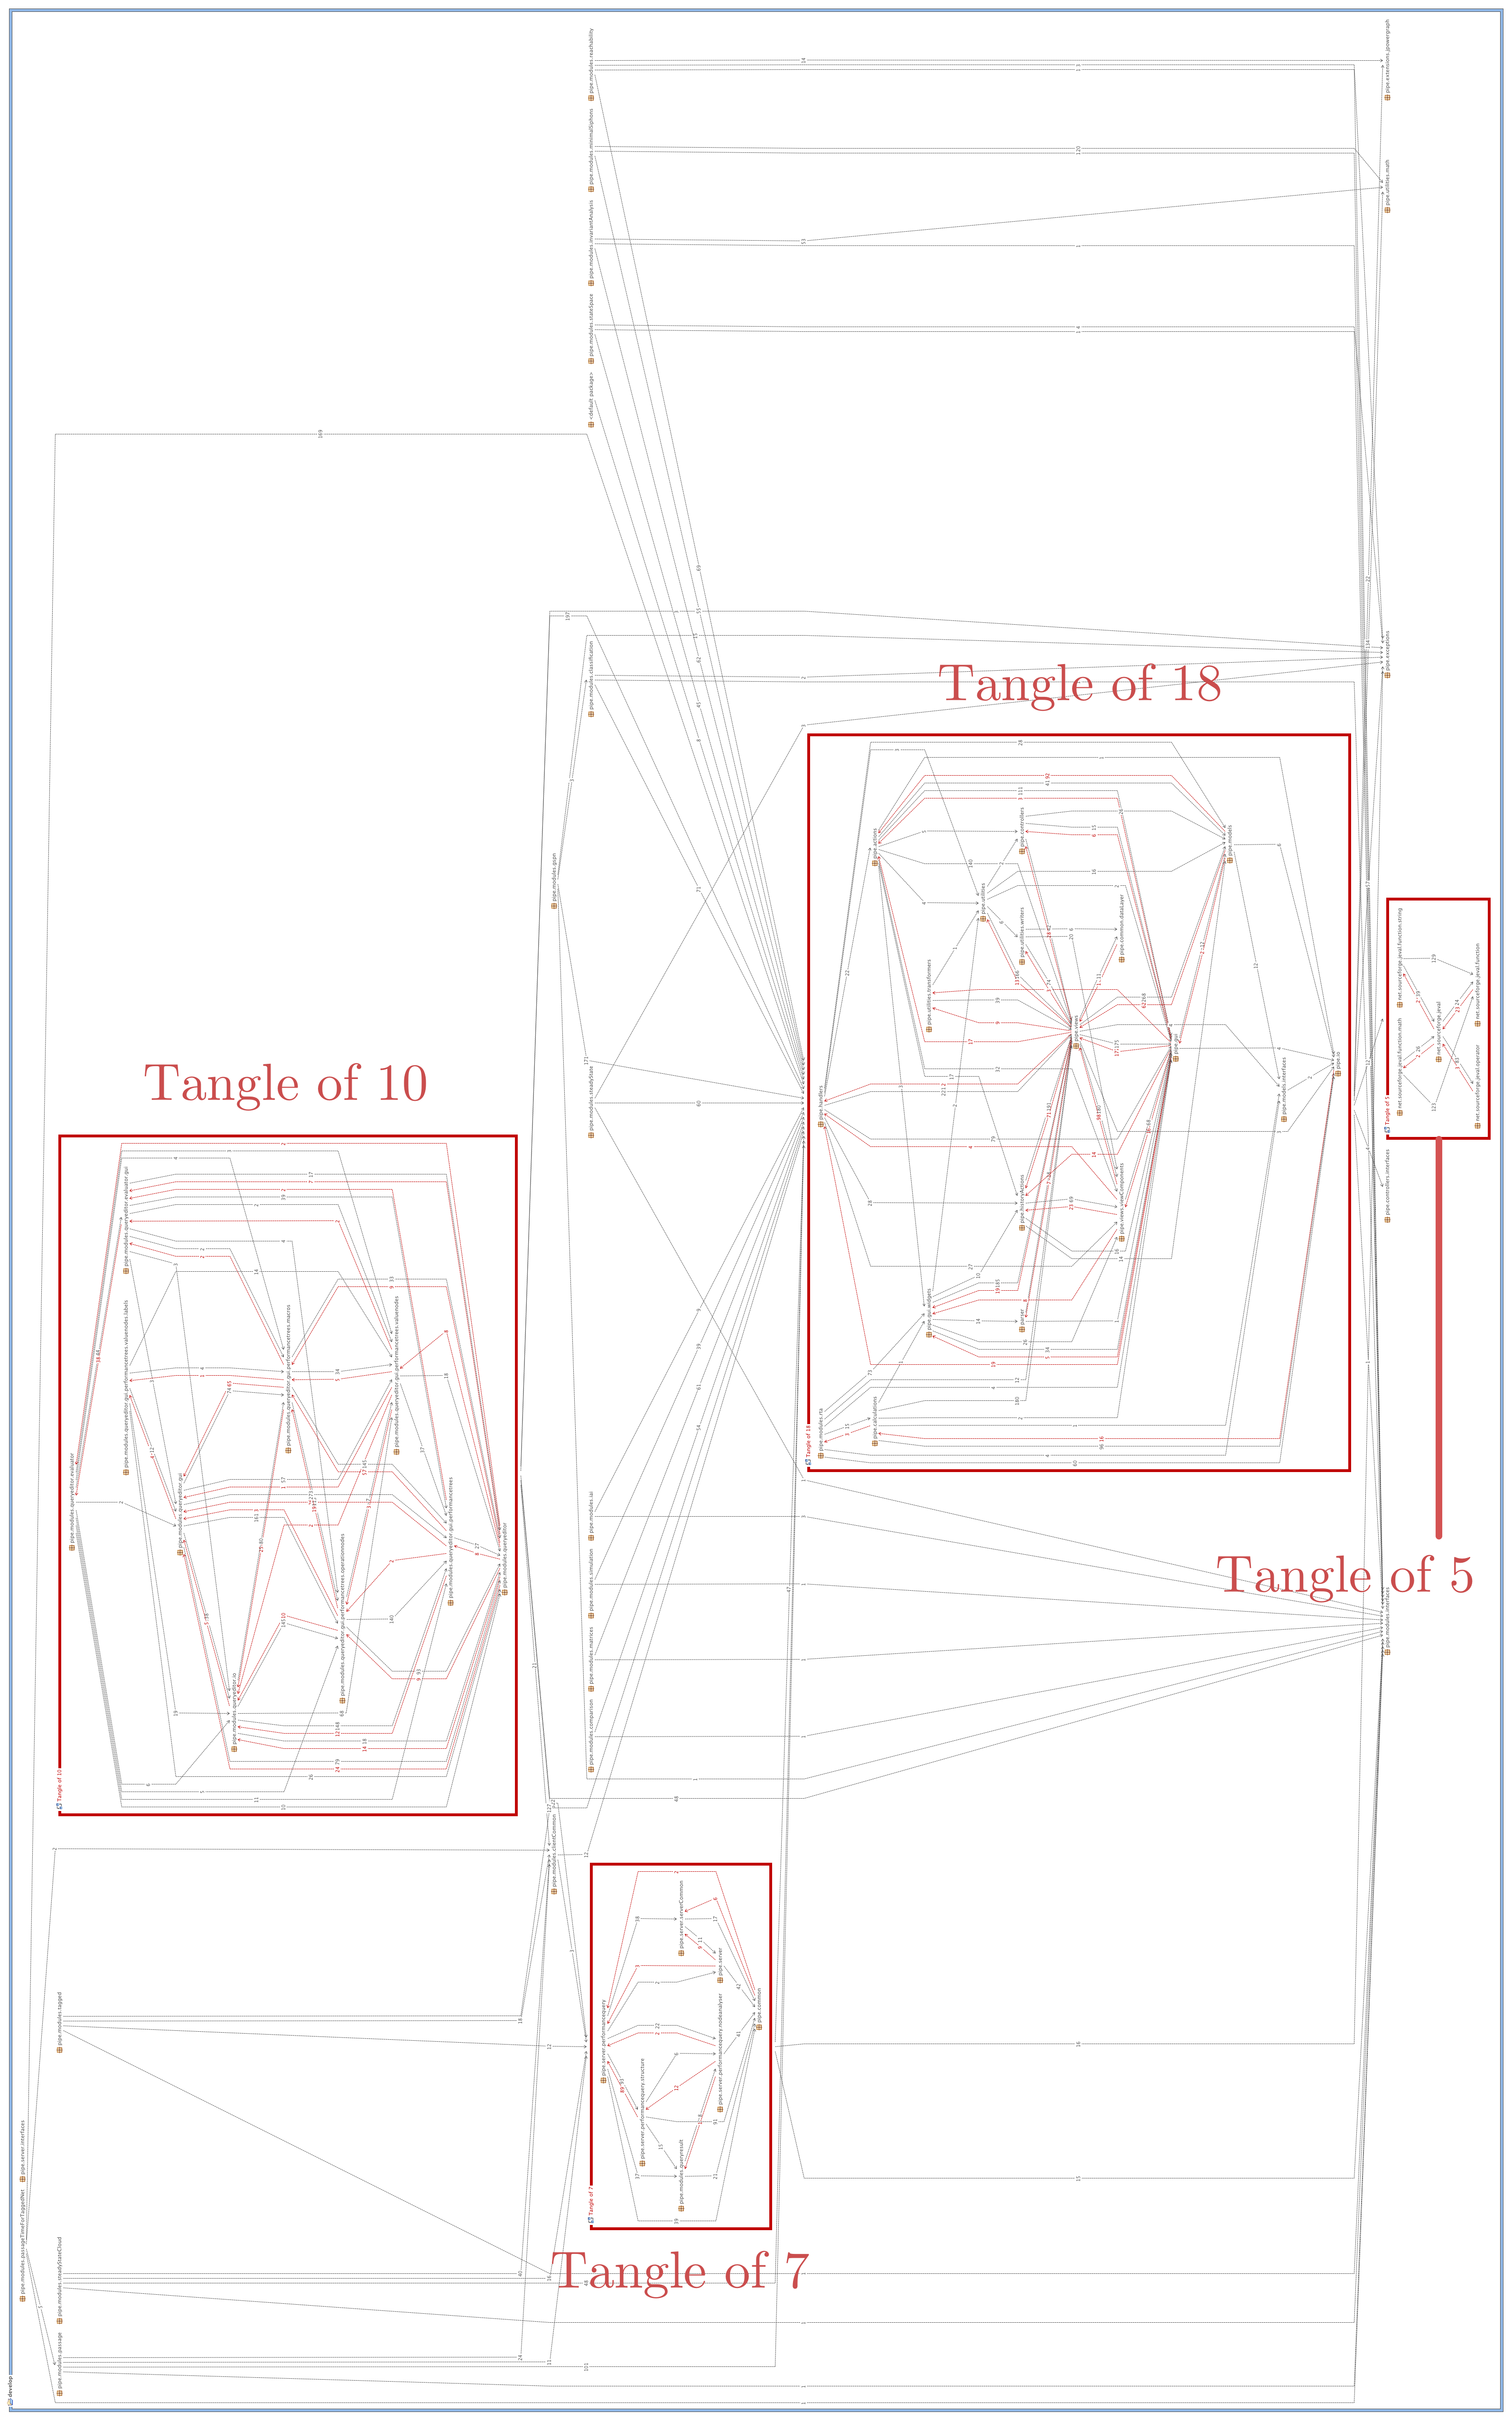
\includegraphics[width=0.8\textwidth]{analysis/tangle_annotated.png} 
    \caption{Stan4J tangle graph of the entire PIPE 4 codebase. It has 4 distinct tangles which are of sizes 18, 10, 7 and 5.}
    \label{fig:tangle}
\end{center}
\end{figure}

% \input{pipe_architecture/standards/tikz/tangle}

% Ideally PIPE should have as few tangles as possible.